\section*{Exercice fil rouge}

Le recueil des besoin de la modélisation du système d'information d'une boulangerie a donné les informations suivantes :

\begin{itemize}
    \item Le boulanger veut connaître ses bénéfices sur la période qu'il désire et archiver ses bilans (ventes - salaires - factures)
\end{itemize}

Lors de ce recueil d'information, les documents suivants ont été jugés utiles :

\begin{itemize}
    \item Ticket de caisse (référence, date, produits, prix)
    \item Fiche de paye (référence, nom, date de naissance et adresse de l'employé, salaire brut)
    \item Bon de commande (nom du fournisseur, date, référence du fournisseur, adresse du fournisseur, produits)
    \item Bon de livraison (nom du fournisseur, date, référence de commande du fournisseur, référence de livraison du fournisseur, produits)
    \item Bon de retour (nom du fournisseur, date, date de livraison, référence de livraison du fournisseur, produits)
    \item Facture (nom du fournisseur, référence du fournisseur, date, prix) \\
\end{itemize}

Autres informations utiles :

\begin{itemize}
    \item on considère qu'une commande est toujours livrée complètement
\end{itemize}


À partir de ces informations le dictionnaire de données et le diagramme de flux suivants ont été élaborés :\\

\begin{figure}[!h]
\begin{tabular}{l l l l l l}
%
    \textbf{mnémonique} & \textbf{desc.} & \textbf{type} & \textbf{format} & \textbf{divers} & \textbf{exemple} \\
    ref-ticket                    & -                & entier  & -            & séquentielle & 1337 \\
    date-ticket                   & -                & date    & jj/mm/aaaa   & -            & 08/10/2016 \\
    nom-produit-vendu             & -                & texte   & 50 car. max. & -            & pain au chocolat \\
    prix-produit-vendu            & -                & décimal & en euros     & -            & 1,20 \\
    quantité-produit-vendu        & -                & décimal & -            & -            & 5.00 \\
    ref-fiche-paye                & -                & entier  & -            & séquentielle & 4237 \\
    nom-employé                   & -                & texte   & 50 car. max. & -            & Jean Dupond \\
    date-naissance-employé        & -                & date    & jj/mm/aaaa   & -            & 06/10/1985 \\
    adresse-employé               & -                & texte   & 75 car. max. & -            & 36 rue des petits pains\\
                                  &                  &         &              &              & 92000 Nanterre \\
    salaire-employé               & -                & décimal & en euros     & -            & 1200,00 \\
    date-paye                     & -                & date    & jj/mm/aaaa   & -            & 08/10/2016 \\
    nom-fournisseur               & -                & texte   & 50 car. max. & -            & Farinin Corp. \\
    date-commande                 & -                & date    & jj/mm/aaaa   & -            & 06/10/2016 \\
    ref-commande-fournisseur      & -                & texte   & 50 car. max. & -            & FC-6102 \\
    adresse-fournisseur           & -                & texte   & 75 car. max. & -            & 120 route de la poudreuse\\
                                  &                  &         &              &              & 92000 Nanterre \\
    nom-produit-acheté            & -                & texte   & 50 car. max. & -            & farine \\
    prix-produit-acheté           & -                & décimal & en euros     & -            & 12,0 \\
    quantité-produit-acheté       & -                & décimal & -            & -            & 50.0 \\
    ref-produit-fournisseur       & -                & texte   & 50 car. max. & -            & FC-6102-farine \\
    date-livraison                & -                & date    & jj/mm/aaaa   & -            & 07/10/2016 \\
    ref-bon-livraison-fournisseur & -                & texte   & 50 car. max. & -            & FC-6102-farine-10 \\
    date-retour                   & -                & date    & jj/mm/aaaa   & -            & 08/10/2016 \\
    ref-facture-fournisseur       & -                & texte   & 50 car. max. & -            & FC-6102-farine-10-fac \\
    date-facturation              & -                & date    & jj/mm/aaaa   & -            & 08/10/2016 \\
    date-paiement                 & -                & date    & jj/mm/aaaa   & -            & 08/10/2016 \\
    date-début                    & -                & date    & jj/mm/aaaa   & -            & 08/10/2015 \\
    date-fin                      & -                & date    & jj/mm/aaaa   & -            & 08/10/2016 \\
%
\end{tabular}
    \caption{\label{DD} Dictionnaire de données}
\end{figure}

\newpage

\begin{figure}[!h]
    \begin{center}
    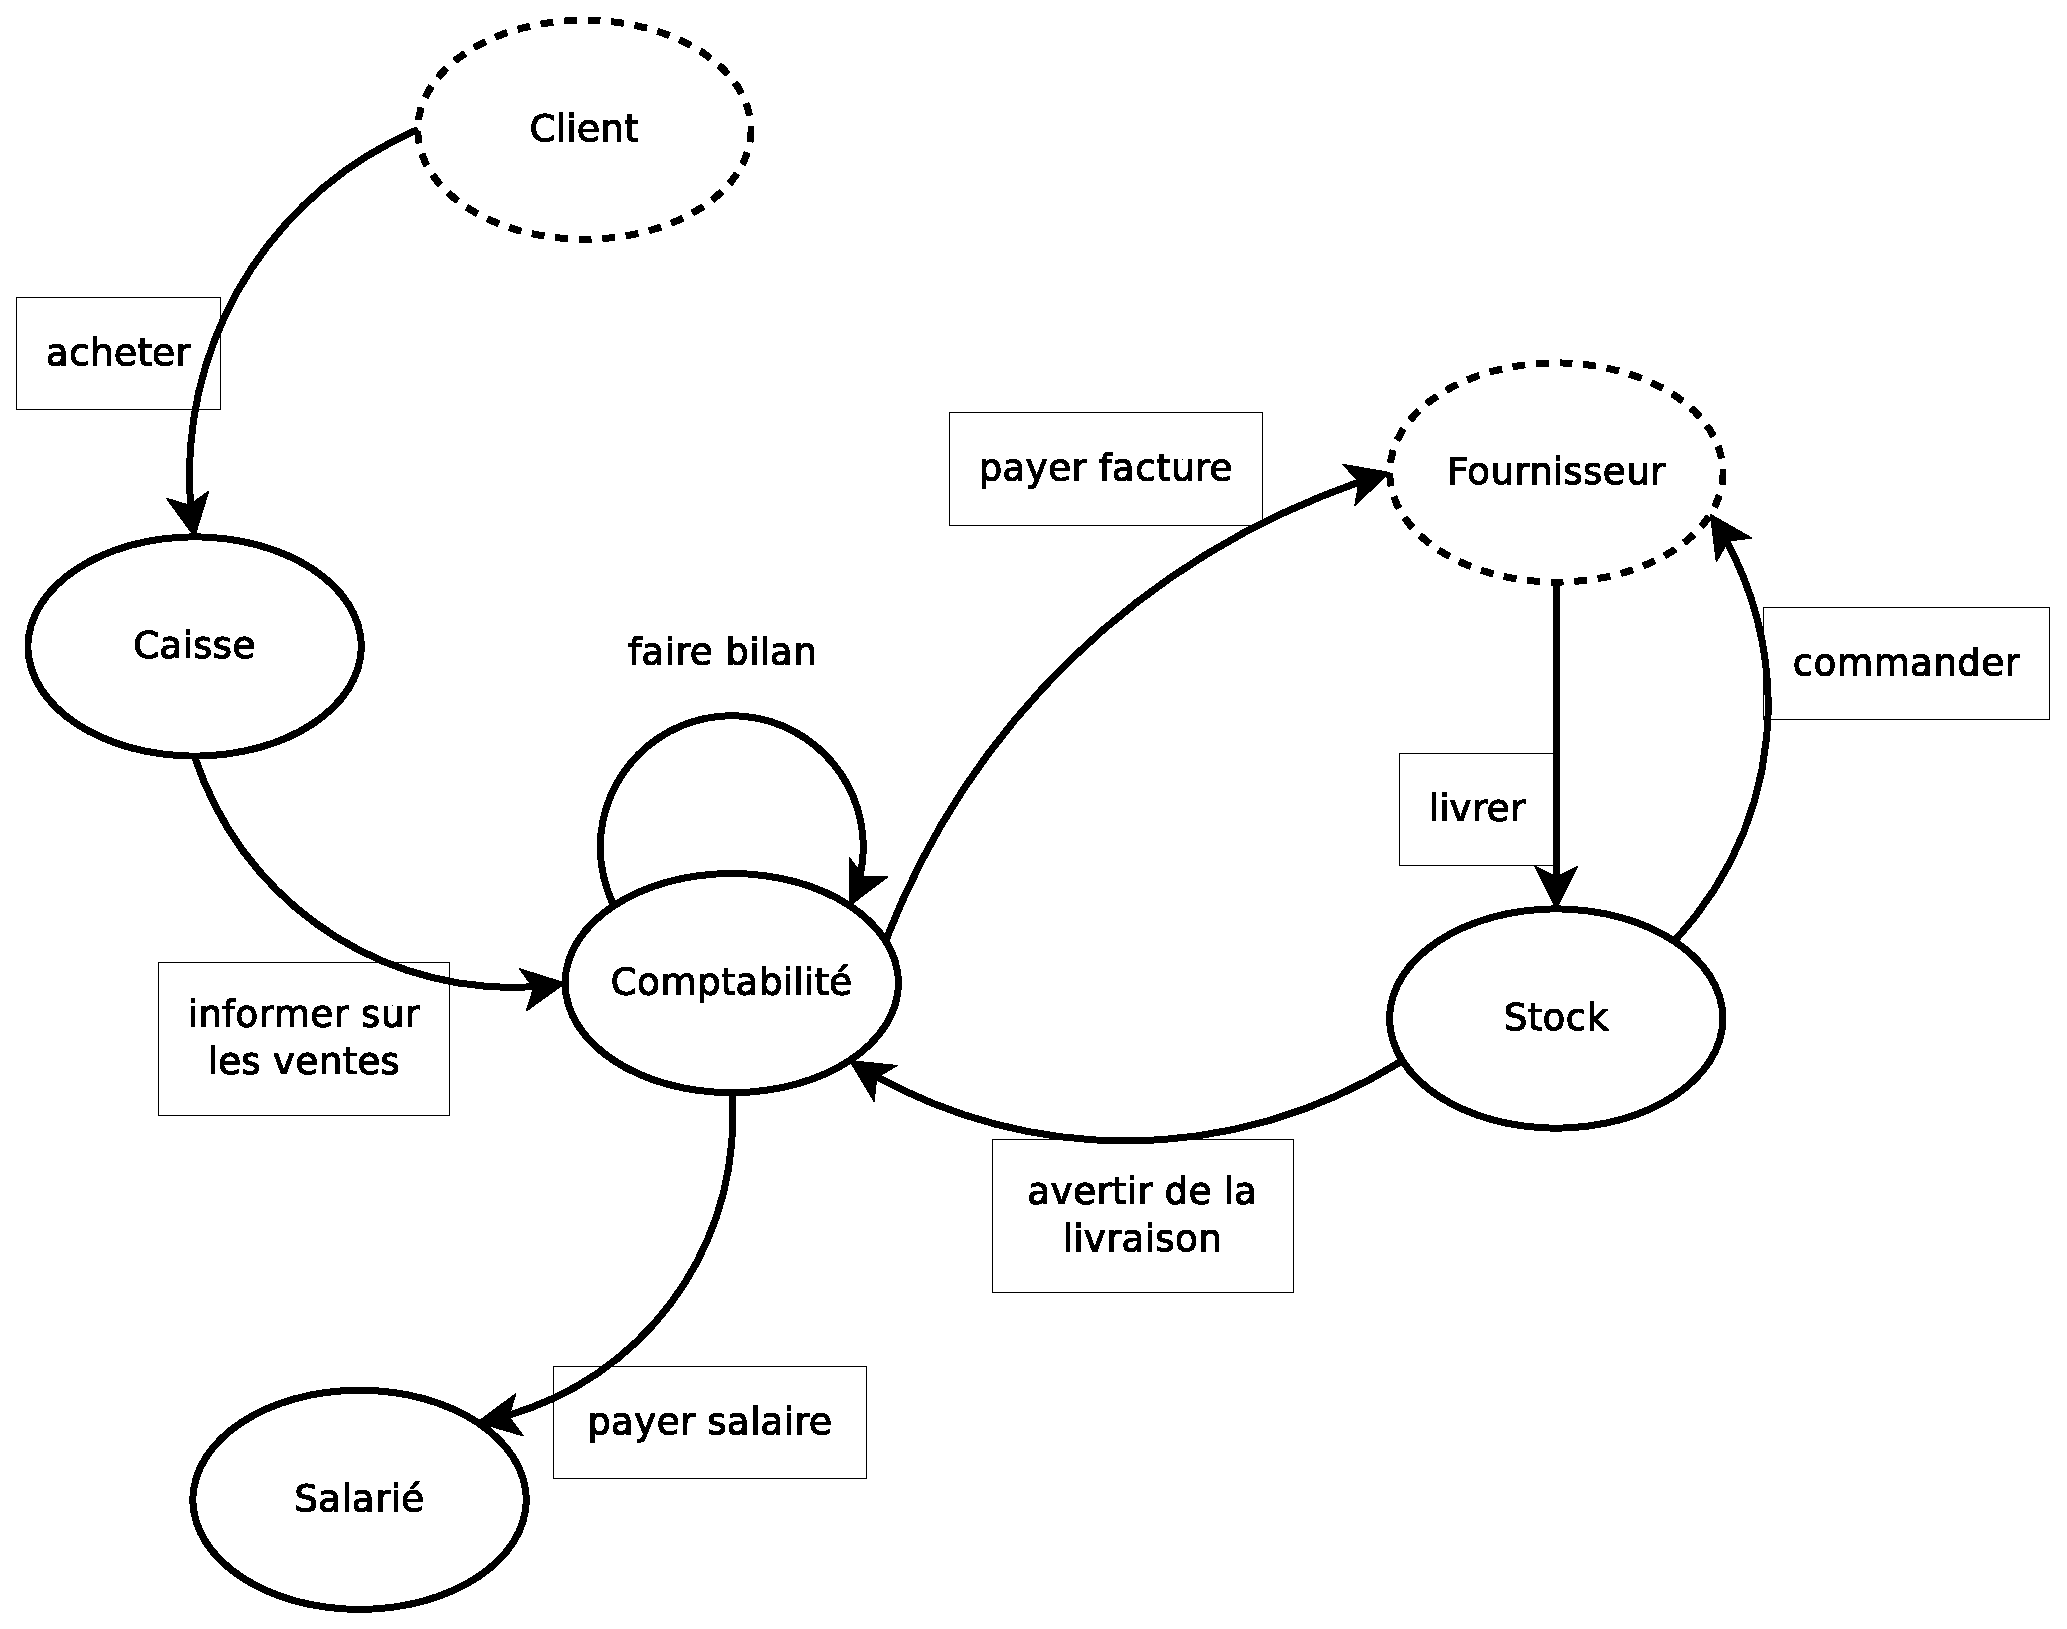
\includegraphics[height=10cm]{images/dd_exo.eps} 
    \caption{\label{DF} Diagramme de Flux}
    \end{center}
\end{figure}

À partir de ces éléments élaborez le modèle conceptuel de communication détaillé (MCC détaillé) puis le modèle conceptuel de données (MCD). Attention, certaines des données utiles peuvent apparaître lors de l'élaboration du modèle conceptuel de données (notamment les références internes des différents éléments).\\

